\subsection*{Finite Element Basis Functions}
\begin{frame}
  % \frametitle{Weighted Residual Statement}
    \begin{columns}[t]
    \column{.5\textwidth}
    \begin{block}{}
%%       \only<1>
%%       {
%% 	To node $i$ we associate a basis function $\psi_i$ such that for any $v^h \in \mathcal{V}^h$
%% 	we have
%% 	\begin{equation}
%% 	  \nonumber
%% 	  v^h = \sum_{i=1}^{N_n} c_i \psi_i
%% 	\end{equation}
%% 	for some constants $c_i$.
%%       }

%%       \only<2>
%%       {
%% 	\begin{itemize}
%% 	  \item{The $\psi_i$ are non-zero only over the elements adjacent to node $i$.}
%% 	  \item{For example, $\psi_i$ could be the linear ``hat'' function.
%% 	    %with value 1
%% 	    %at node $i$ and zero at all other nodes.
%% 	  }
%% 	\end{itemize}
%%       }

%%       \only<3->
%%       {
	\begin{itemize}
	  \item{An element integral will have contributions only
	    from the global basis functions corresponding to its nodes.}
	  \item{We call these local basis functions $\phi_i$, $0 \leq i \leq N_s$.}
	\end{itemize}
%%      }
    \end{block}

%%       \visible<3->
%%       {
	    \begin{equation}
	      \nonumber
	      \left. v^h \right|_{\Omega_e} = \sum_{i=1}^{N_s} c_i \phi_i
	    \end{equation}
%%      }
      \visible<2>
      {
	    \begin{equation}
	      \nonumber
	      \alert{\int_{\Omega_e}} v^h \;\alert{dx}
	      = \sum_{i=1}^{N_s} c_i \alert{\int_{\Omega_e}}\phi_i \;\alert{dx}
	    \end{equation}

      }
%}
%  \end{itemize}
    \column{.5\textwidth}
    %\begin{block}{}
      \begin{center}
%% 	\only<1>
%% 	    {
%% 	      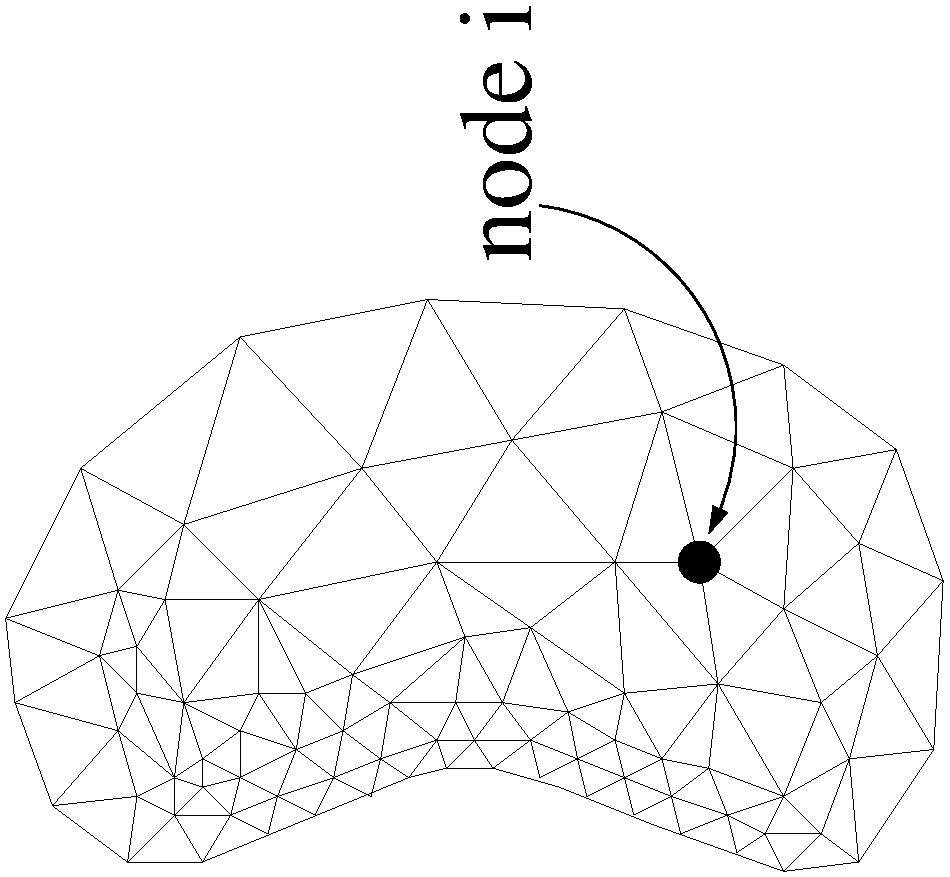
\includegraphics[width=2in,angle=-90]{node_i}
%% 	    }
%% 	\only<2>
%% 	    {
%% 	      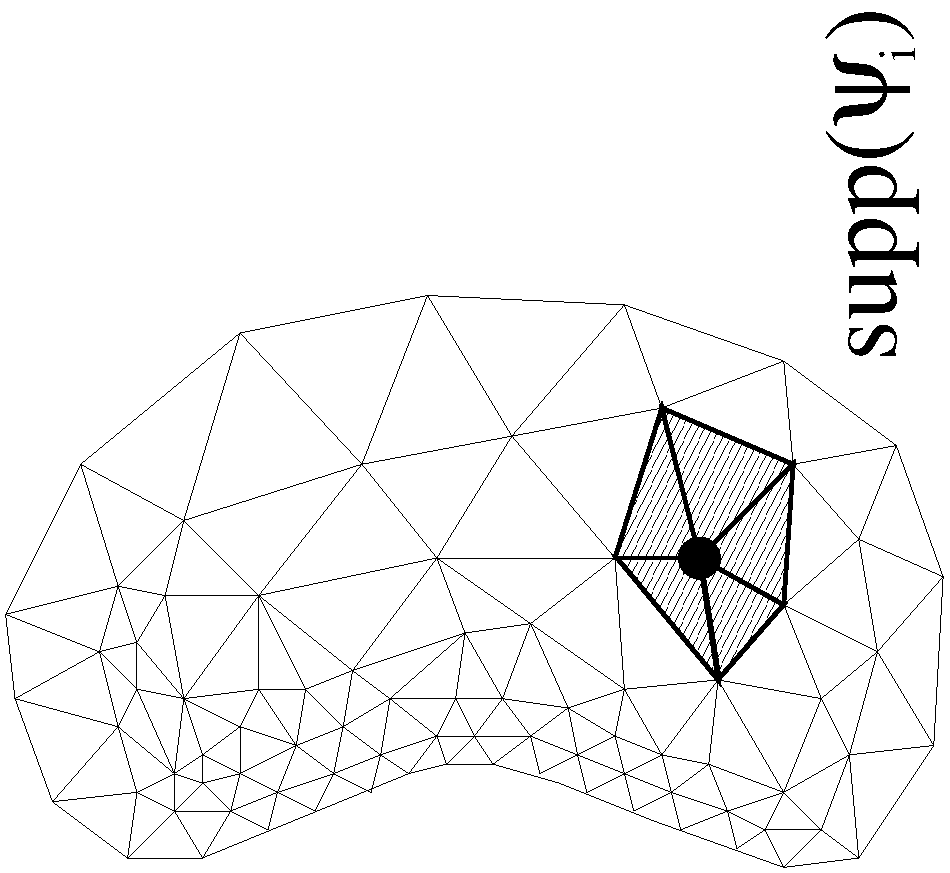
\includegraphics[width=2in,angle=-90]{phi_i}
%% 	    }
%% 	\only<3->
%% 	    {
	      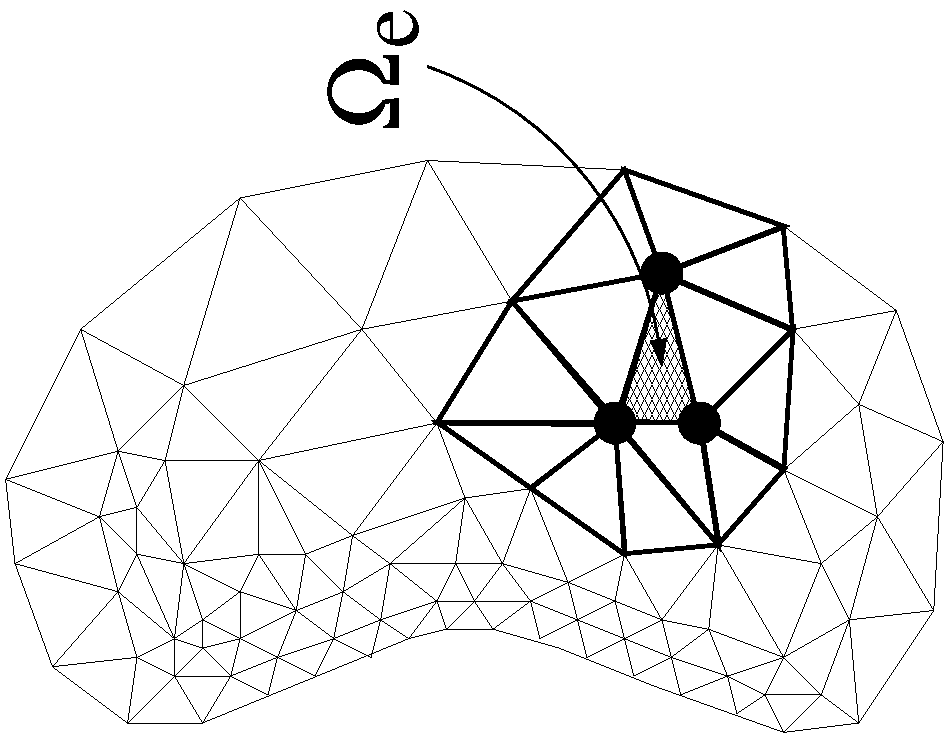
\includegraphics[width=2in,angle=-90]{phi_ijk}
%%	    }
      \end{center}
    \end{columns}
\end{frame}
